\documentclass[10pt]{beamer}

%%%
% PREAMBLE FOR THIS DOC 
%%%
%https://tex.stackexchange.com/questions/68821/is-it-possible-to-create-a-latex-preamble-header
\usepackage{/Users/miw267/Repos/csci246_spring2025/slides/preambles/beamer_preamble_for_CSCI246}



%%% TRY TO RESHOW TOC AT EACH SECTION START (with current section highlighted)
% Reference: https://tex.stackexchange.com/questions/280436/how-to-highlight-a-specific-section-in-beamer-toc
\newcommand\tocforsect[2]{%
  \begingroup
  \edef\safesection{\thesection}
  \setcounter{section}{#1}
  \tableofcontents[#2,currentsection]
  \setcounter{section}{\safesection}
  \endgroup
}


%%%% HERES HOW TO DO IT CORRECTLY
% FIRST IN .STY FILE, DO
%\usetheme[sectionpage=none]{metropolis}
% THEN AT EACH SECTION DO
%\begin{frame}{Outline}
%  \tableofcontents[currentsection]	
%\end{frame}



%\setbeamertemplate{navigation symbols}{}
%\setbeamertemplate{footline}[frame number]{}


%%%
% DOCUMENT
%%%

\begin{document}

%\maketitle

%% Title page frame
%\begin{frame}
%    \titlepage 
%\end{frame}





\title{03/03/2025: Functions}
\author{CSCI 246: Discrete Structures}
\date{Textbook reference: Sec 24, Scheinerman}

\begin{frame}
    \titlepage 
\end{frame}


\begin{frame}
\footnotesize 
\begin{mygreenbox}[title=Graded Quiz Pickup]
Quizzes are in the front of the room, grouped into four bins (A-G, H-L, M-R, S-Z) by last name. The quizzes are upside down with your last name on the back. Come find yours before, during, or after class.  Only turn the quiz over if it's yours.
\end{mygreenbox} 
\vfill 

\begin{myredbox}[title=Announcement: How to be sure you're reading the right section]
\begin{enumerate}
	\item Check the current version of the syllabus to confirm the reading for the \textbf{next} course meeting sometime during (or after) class.  
	\item The most current version of the syllabus can always be found at the \href{https://github.com/mikewojnowicz/csci246_spring2025}{course repo}.  
\end{enumerate}
\end{myredbox}

\vfill 


\begin{myyellowbox}[title=Today's Agenda]
\begin{itemize}
	\item Reading quiz (5 mins)
	\item Mini-lecture ($\approx$ 25 mins)
%	%
%	\begin{itemize}
%	\footnotesize 
%	\item Review induction 
%	\end{itemize}
%	%
	\item Group exercises ($\approx$ 15 mins)
\end{itemize}

%	Rationale for group exercises: we got shortchanged on time last couple days, and I already did a lot of lectures, so I want you to practice. Next problems quiz will cover relations and functions: Hamkins and 
%	
\end{myyellowbox}
\vfill 

\end{frame}

\begin{frame}[standout]
Feedback on Friday's Quizzes 
\end{frame}



\begin{frame}{Scores On Reading Quiz (Partitions)(Extra Credit)}
\footnotesize 
\begin{figure}[ht]
        \centering
        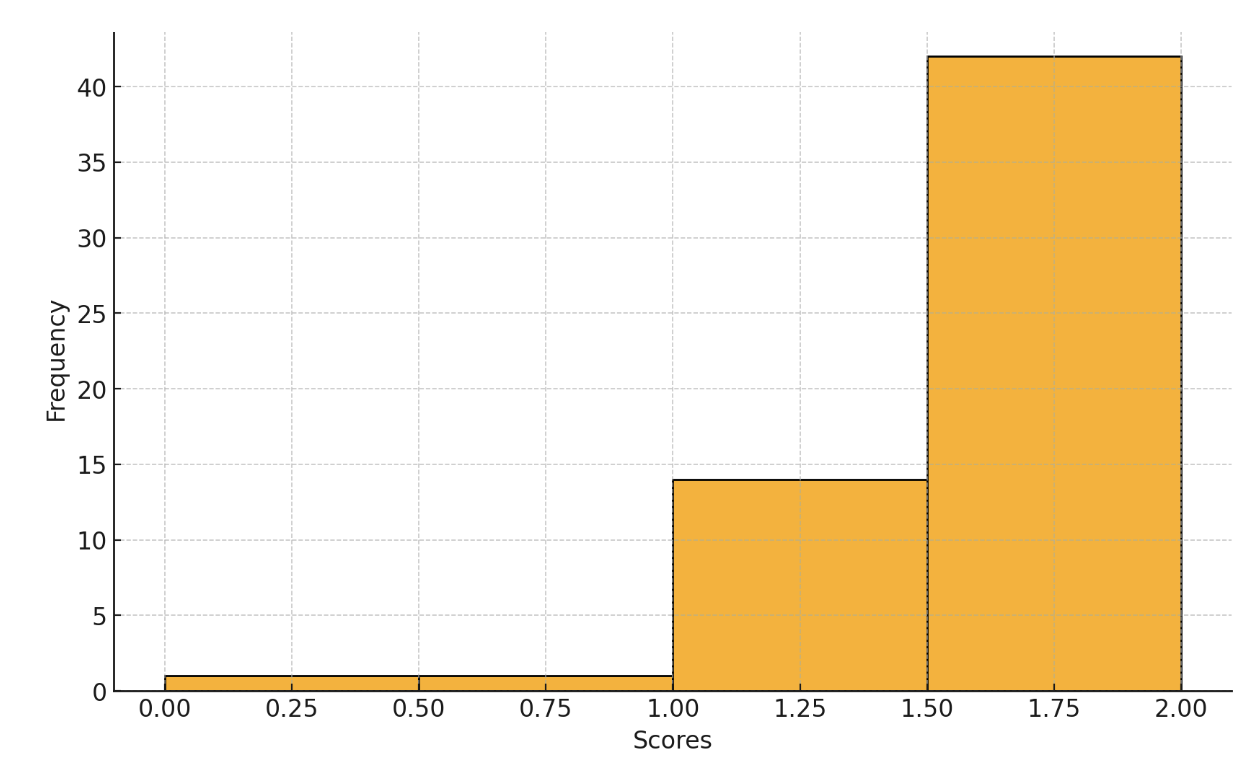
\includegraphics[width=.7\textwidth]{images/reading_quiz_scores}
   		 \caption{Median Score = 1.75/2 (87.5\%)}
\end{figure}
\vfill 
\textbf{Rubric.}  	
\begin{itemize}
\item  1 point if correct.  Any partition works.  The first page of the text has 3 examples.
\item 1 point if correct.  The correct solution is 8!/(3!2!)
\end{itemize}
\end{frame}


\begin{frame}{Scores On Problems Quiz (Relations)}
\footnotesize 
\begin{figure}[ht]
        \centering
        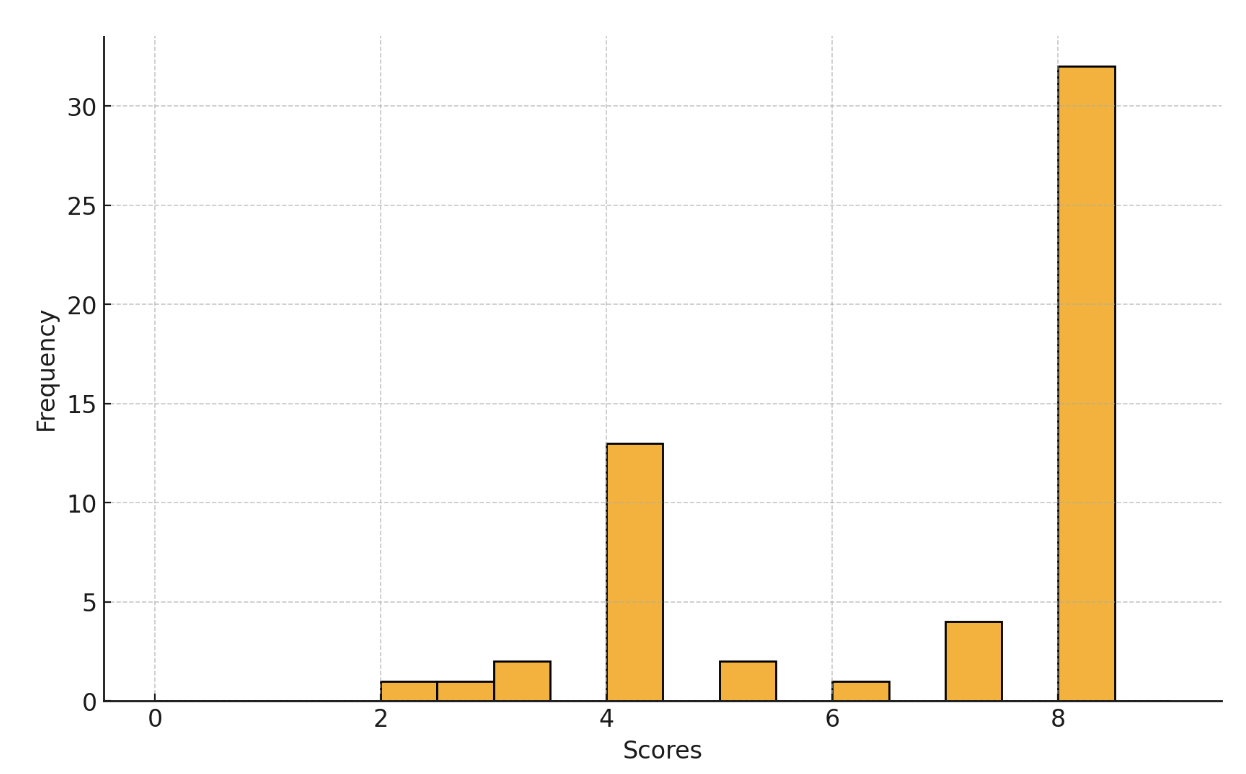
\includegraphics[width=.6\textwidth]{images/problem_quiz_scores}
   		 \caption{Median Score = 8/8 (100\%)}
\end{figure}
\vfill 
\textbf{Rubric.}  	
\begin{itemize}
\item  (4 points) 4 point for an example that is correct.  See group exercises from the relations day for one example.
\item (4 points) 1 point for correct answer (yes, it’s an equivalence relation), 1 point for naming a property that is one of the 3 properties of an equivalence relation (transitivity, reflexivity, and symmetry), and 2 points for a correct proof.
\end{itemize}
\end{frame}


\begin{frame}
\begin{minipage}{0.63\textwidth}
 \begin{myredbox}[title=Reading Quiz (Functions)]
 Let $A = \set{0,1,2,3,4}$ and $B=\set{5,6,7,8,9}$. Let $f: A \to B$ be defined by
 \[  f= \set{(0,5), (1,7), (2,8), (3,9), (4,7)}\]
 So 
 \[ f^{-1} = \set{(5,0), (7,1), (8,2), (9,3), (7,4)}\]  
 
 The figure on top shows $f$, and the figure on the bottom shows $f^{-1}$.
 
\begin{enumerate}
	\item Is $f^{-1}$ a function from $B$ to $A$?
	\item Give one reason for your answer to \#1 .
	\item (Extra credit.) Give a second reason for your answer to \#2.
\end{enumerate}
\end{myredbox}
\end{minipage}
\hfill 
\begin{minipage}{0.35\textwidth}
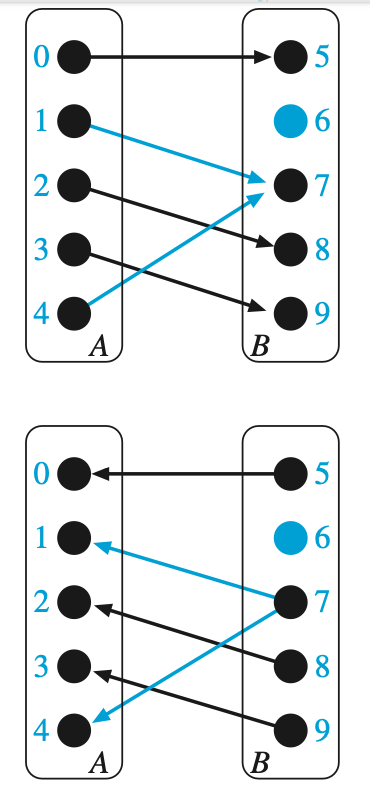
\includegraphics[width=0.8\textwidth]{images/reading_quiz_plot.png}	
\end{minipage}
\end{frame}


\begin{frame}[standout]
Q  \& A on Group Exercises  (Equivalence Relations and Partitions)
\end{frame}


\begin{frame}[standout]
Overview of functions
\end{frame}


\begin{frame}


\begin{myyellowbox}[title=Remark]
A function is a special type of a binary relation.
\end{myyellowbox}

\vfill 
\begin{mygreenbox}[title=Definition (Hampkins pp. 128)]
We say that $f$ is \textbf{function} from $A$ to $B$, written $f : A \to B$, if $f$ is a set of pairs $ f \subseteq  A \times B$ exhibiting the \underline{function property}: for every $a \in A$, there is a unique $b \in B$ with $(a, b) \in f$. This object $b$ is denoted by $f(a)$ and is called the value of the function at $a$.
\end{mygreenbox}
\vfill 
\begin{myredbox}[title=Characterization]
We can think of a \textbf{function} as a rule that assigns each element of a set $A$ to \underline{exactly one} element in another set $B$.
\end{myredbox}

\end{frame}


\begin{frame}

\begin{myredbox}[title=Characterization]
We can think of a \textbf{function} as a rule that assigns each element of a set $A$ to \underline{exactly one} element in another set $B$.
\end{myredbox}
\vfill 
\begin{myyellowbox}[title=Poll]

Let $A=\set{a,b,c,d}$ and $B=\set{e,f,g}$. Consider a relation $R$ depicted below.

\begin{center}
\begin{tikzpicture}

% Nodes in a vertical line
\node[latent] (A1) at (-2, 3) {a};
\node[latent] (A2) at (-2, 2) {b};
\node[latent] (A3) at (-2, 1) {c};
\node[latent] (A4) at (-2, 0) {d};
\node[latent] (B2) at (1, 2) {e};
\node[latent] (B3) at (1, 1) {f};
\node[latent] (B4) at (1, 0) {g};


% Edges
\path[->, >=stealth] (A1) edge (B2);
\path[->, >=stealth] (A2) edge (B2);
\path[->, >=stealth] (A3) edge (B3);
\path[->, >=stealth] (A4) edge (B2);
%\path[->, >=stealth] (A4) edge (B3);
%\path[->, >=stealth] (A4) edge (B4);
\end{tikzpicture}
\end{center}
Is $R$ a function? \pause Yes.
\end{myyellowbox}
	
\end{frame}




\begin{frame}

\begin{myredbox}[title=Characterization]
We can think of a \textbf{function} as a rule that assigns each element of a set $A$ to \underline{exactly one} element in another set $B$.
\end{myredbox}
\vfill 
\begin{myyellowbox}[title=Poll]

Let $A=\set{a,b,c,d}$ and $B=\set{e,f,g}$. Consider a relation $R$ depicted below.

\begin{center}
\begin{tikzpicture}

% Nodes in a vertical line
\node[latent] (A1) at (-2, 3) {a};
\node[latent] (A2) at (-2, 2) {b};
\node[latent] (A3) at (-2, 1) {c};
\node[latent] (A4) at (-2, 0) {d};
\node[latent] (B2) at (1, 2) {e};
\node[latent] (B3) at (1, 1) {f};
\node[latent] (B4) at (1, 0) {g};



% Edges
\path[->, >=stealth] (A1) edge (B2);
\path[->, >=stealth] (A2) edge (B2);
\path[->, >=stealth] (A3) edge (B3);
%\path[->, >=stealth] (A4) edge (B2);
%\path[->, >=stealth] (A4) edge (B3);
%\path[->, >=stealth] (A4) edge (B4);
\end{tikzpicture}
\end{center}
Is $R$ a function? \pause No. Element $d$ does not get mapped to anything.
\end{myyellowbox}
	
\end{frame}



\begin{frame}

\begin{myredbox}[title=Characterization]
We can think of a \textbf{function} as a rule that assigns each element of a set $A$ to \underline{exactly one} element in another set $B$.
\end{myredbox}
\vfill 
\begin{myyellowbox}[title=Poll]

Let $A=\set{a,b,c,d}$ and $B=\set{e,f,g}$. Consider a relation $R$ depicted below.

\begin{center}
\begin{tikzpicture}

% Nodes in a vertical line
\node[latent] (A1) at (-2, 3) {a};
\node[latent] (A2) at (-2, 2) {b};
\node[latent] (A3) at (-2, 1) {c};
\node[latent] (A4) at (-2, 0) {d};
\node[latent] (B2) at (1, 2) {e};
\node[latent] (B3) at (1, 1) {f};
\node[latent] (B4) at (1, 0) {g};



% Edges
\path[->, >=stealth] (A1) edge (B2);
\path[->, >=stealth] (A2) edge (B2);
\path[->, >=stealth] (A3) edge (B3);
\path[->, >=stealth] (A4) edge (B2);
\path[->, >=stealth] (A4) edge (B3);
%\path[->, >=stealth] (A4) edge (B4);
\end{tikzpicture}
\end{center}
Is $R$ a function? \pause No. Element $d$ gets mapped to \underline{both} $e$ and $f$.
\end{myyellowbox}
	
\end{frame}

\begin{frame}[standout]
Domain, co-domain, and range	
\end{frame}


\begin{frame}
\footnotesize 
\begin{mygreenbox}[title=Definitions (Hampkins pp. 128)]
Let $f$ be a function from $A$ to $B$.  We call $A$ the \textbf{domain} of the function, and we call $B$ the \textbf{codomain} (or \textbf{target}) of the function.   \\

The \textbf{range} (or \textbf{image}) of  the function, in contrast, is the set of all $b$ that arise as $f(a)$ for some $a$ in the domain. (It is the set of all elements in 
$B$ that are actually \enquote{hit} by $f$).

\end{mygreenbox}
 
\vfill 
\begin{myyellowbox}[title=Poll]

Let $A=\set{a,b,c,d}$ and $B=\set{e,f,g}$. Consider the function below.

\begin{center}
\begin{tikzpicture}[scale=0.7]

% Nodes in a vertical line
\node[latent] (A1) at (-2, 3) {a};
\node[latent] (A2) at (-2, 2) {b};
\node[latent] (A3) at (-2, 1) {c};
\node[latent] (A4) at (-2, 0) {d};
\node[latent] (B2) at (1, 2) {e};
\node[latent] (B3) at (1, 1) {f};
\node[latent] (B4) at (1, 0) {g};


% Edges
\path[->, >=stealth] (A1) edge (B2);
\path[->, >=stealth] (A2) edge (B2);
\path[->, >=stealth] (A3) edge (B3);
\path[->, >=stealth] (A4) edge (B2);
%\path[->, >=stealth] (A4) edge (B3);
%\path[->, >=stealth] (A4) edge (B4);
\end{tikzpicture}
\end{center}


What are the domain, codomain and range? \pause The domain is  $A=\set{a,b,c,d}$, the codomain is and $B=\set{e,f,g}$, and the range is $\set{e,f}$. Note that the range is smaller than $B$.
\end{myyellowbox}
	
\end{frame}


\begin{frame}[standout]
Injectivity and surjectivity
\end{frame}


\begin{frame}

\footnotesize 
\begin{mygreenbox}[title=Definitions (Hampkins pp. 128)]
%A function $f : A \to B$ is said to be  \textbf{surjective} (or \textbf{onto}) if for all $b \in B$, there is $a \in A$ such that $f(a)=b$. In other words, the range of $f$ is all of $B$. \\
A function $f : A \to B$ is said to be  \textbf{surjective} (or \textbf{onto}) if the range of $f$ is all of $B$.  (That is, all of $B$ is \enquote{hit} by the function.)\\
\vfill 
The function $f$  is said to be  \textbf{injective} (or \textbf{one-to-one}) if whenever $a \neq a'$, we have $f(a) \neq f(a')$.  (That is, distinct inputs always lead to distinct outputs.) \\
\vfill The function $f$ is said to be \textbf{bijective} if it is both surjective and injective.	
\end{mygreenbox}
 
\vfill 

\begin{myyellowbox}[title=Poll]
	\centering
	\resizebox{\textwidth}{!}{%
    \begin{tabular}{ccccc}
       \onslide<1->{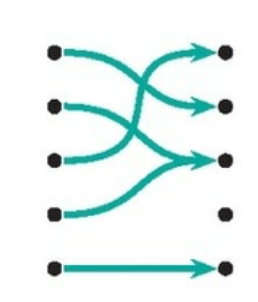
\includegraphics[width=0.2\textwidth]{images/f1.png}} & \onslide<3->{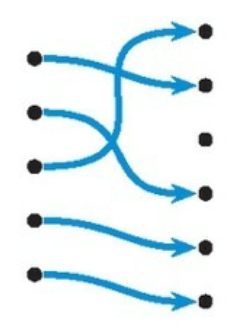
\includegraphics[width=0.2\textwidth]{images/f2.png}} & \onslide<5->{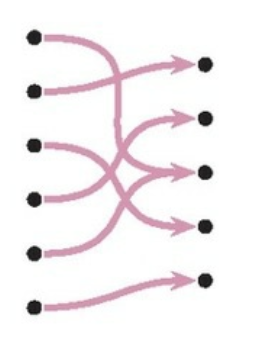
\includegraphics[width=0.2\textwidth]{images/f3.png}}  & \onslide<7->{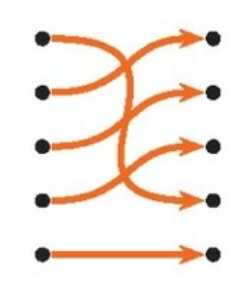
\includegraphics[width=0.2\textwidth]{images/f4.png}}  & \onslide<9->{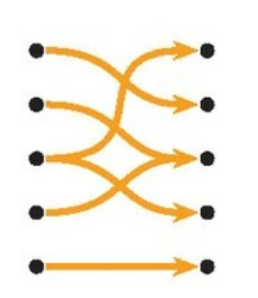
\includegraphics[width=0.2\textwidth]{images/f5.png}} \\
        \onslide<2->{Not injective} & \onslide<4->{Injective} & \onslide<6->{Not injective} & \onslide<8->{Injective} & \onslide<10->{Not a function}\\
           \onslide<2->{Not surjective} & \onslide<4->{Not surjective} & \onslide<6->{Surjective} & \onslide<8->{Surjective} & \onslide<10->{}\\
    \end{tabular}
    }
\end{myyellowbox}
\end{frame}


\begin{frame}[standout]
Inverse functions
\end{frame}


\begin{frame}

\footnotesize 
\begin{mygreenbox}[title=Definition (Scheinerman Def. 14.4)]
Let $R$ be a relation.  The \textbf{inverse relation} of $R$, denoted $R^{-1}$, is the relation formed by reversed the order of all the ordered pairs of $R$.
\end{mygreenbox}
 
\vfill 

\begin{myredbox}[title=Theorem (Scheinerman Thm 24.21)]
Let $A$ and $B$ be sets and let $f: A \to B$.   The inverse relation $f^{-1}$ is a \textit{function} from $B$ to $A$ if and only if $f$ is a bijection.
	
\end{myredbox}
\vfill 

\begin{myyellowbox}[title=Poll]
	\centering
	\resizebox{\textwidth}{!}{%
    \begin{tabular}{ccccc}
     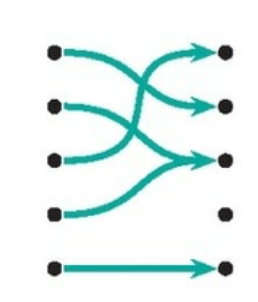
\includegraphics[width=0.2\textwidth]{images/f1.png} & 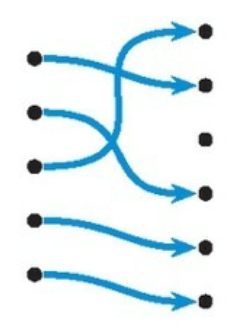
\includegraphics[width=0.2\textwidth]{images/f2.png} & 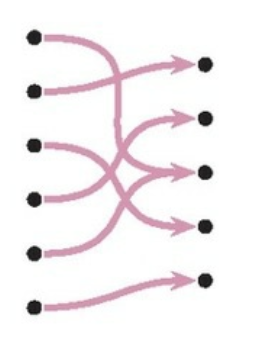
\includegraphics[width=0.2\textwidth]{images/f3.png}  & 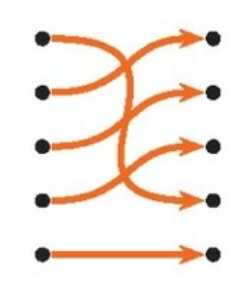
\includegraphics[width=0.2\textwidth]{images/f4.png}  & 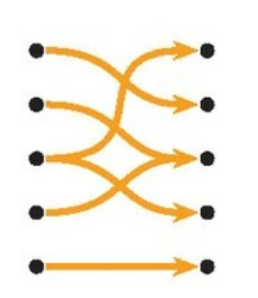
\includegraphics[width=0.2\textwidth]{images/f5.png} \\
        Not injective & Injective & Not injective & Injective & Not a function\\
           Not surjective & Not surjective & Surjective & Surjective & \\
    \end{tabular}
    } \\
    
   \vspace{0.5cm} 
For which relations $f$ above is $f^{-1}$ a function? Why or why not?
\end{myyellowbox}
\end{frame}


\begin{frame}
\begin{minipage}{0.63\textwidth}
 \begin{myredbox}[title=Solution to reading quiz]
 Let $A = \set{0,1,2,3,4}$ and $B=\set{5,6,7,8,9}$. Let $f: A \to B$ be defined by
 \[  f= \set{(0,5), (1,7), (2,8), (3,9), (4,7)}\]
 So 
 \[ f^{-1} = \set{(5,0), (7,1), (8,2), (9,3), (7,4)}\]  
 
Is $f^{-1}$ a function from $B$ to $A$? \pause 
No, $f$ is not bijective.  In particular:
 
\begin{enumerate}
	\item $f$ is not surjective.  So the input $6$ doesn't map to \textit{any} outputs.
	\item $f$ is not injective.  So the input $7$ maps to \textit{multiple} outputs.
\end{enumerate}
\end{myredbox}
\end{minipage}
\hfill 
\begin{minipage}{0.35\textwidth}
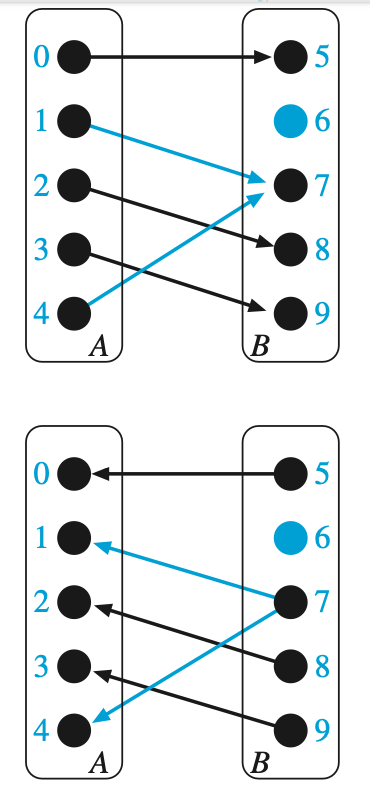
\includegraphics[width=0.8\textwidth]{images/reading_quiz_plot.png}	
\end{minipage}
\end{frame}


\begin{frame}[standout]
Group exercises
\end{frame}

\begin{frame}
\footnotesize 
\vfill 
\begin{columns}
\begin{column}{0.33\textwidth}
aaron.loomis: 20 \\ 
adam.wyszynski: 18 \\ 
alexander.goetz: 9 \\ 
alexander.knutson: 1 \\ 
anthony.mann: 4 \\ 
blake.leone: 5 \\ 
bridger.voss: 21 \\ 
caitlin.hermanson: 1 \\ 
cameron.wittrock: 5 \\ 
carsten.brooks: 6 \\ 
carver.wambold: 5 \\ 
colter.huber: 13 \\ 
conner.reed1: 1 \\ 
connor.mizner: 8 \\ 
connor.yetter: 16 \\ 
derek.price4: 12 \\ 
devon.maurer: 2 \\ 
emmeri.grooms: 10 \\ 
erik.moore3: 21 \\ 
ethan.johnson18: 17 \\ 
evan.barth: 11 \\\end{column}
\begin{column}{0.33\textwidth}
evan.schoening: 19 \\ 
griffin.short: 20 \\ 
jack.fry: 11 \\ 
jacob.ketola: 14 \\ 
jacob.ruiz1: 13 \\ 
jacob.shepherd1: 17 \\ 
jada.zorn: 16 \\ 
jakob.kominsky: 10 \\ 
james.brubaker: 16 \\ 
jeremiah.mackey: 12 \\ 
jett.girard: 14 \\ 
john.fotheringham: 2 \\ 
jonas.zeiler: 8 \\ 
joseph.mergenthaler: 7 \\ 
joseph.triem: 10 \\ 
julia.larsen: 9 \\ 
justice.mosso: 8 \\ 
kaden.price: 19 \\ 
lucas.jones6: 19 \\ 
luka.derry: 13 \\ 
luke.donaldson1: 2 \\\end{column}
\begin{column}{0.33\textwidth}
lynsey.read: 15 \\ 
mason.barnocky: 7 \\ 
matthew.nagel: 18 \\ 
micaylyn.parker: 14 \\ 
michael.oswald: 3 \\ 
nolan.scott1: 3 \\ 
owen.obrien: 4 \\ 
pendleton.johnston: 20 \\ 
peter.buckley1: 6 \\ 
reid.pickert: 15 \\ 
ryan.barrett2: 6 \\ 
samuel.hemmen: 15 \\ 
samuel.mosier: 4 \\ 
samuel.rollins: 17 \\ 
sarah.periolat: 11 \\ 
timothy.true: 3 \\ 
tristan.nogacki: 21 \\ 
tyler.broesel: 7 \\ 
william.elder1: 18 \\ 
yebin.wallace: 9 \\ 
zeke.baumann: 12 \\\end{column}
\end{columns}
\vfill
\end{frame}


\begin{frame}{Group exercises}
\footnotesize 
\begin{enumerate}
	\item Let $A =\set{1,2,3,4}$ and $B=\set{5,6,7}$.  Let $f$ be the relation
	\[  f=\set{(1,5),(2,5), (3,6),(?,?)}\]
	Find replacements for (?,?) so that each of the following is true.
	\begin{itemize} \footnotesize 
		\item [a.] The relation $f$ is not a function from $A$ to $B$.
		\item [b.] The relation $f$ is a function from $A$ to $B$ but is not onto $B$.
		\item [c.] The relation $f$ is a function from $A$ to $B$ and is onto $B$.
	\end{itemize}
	\item Let $f: \mathbb{Z} \to \mathbb{N}$ by $f(x)=|x|$.   (a) Is $f$ one-to-one? (b) Is $f$ onto?
	\item Consider the \enquote{shifting} (or translation) function $f: \mathbb{Z} \to \mathbb{Z}$ given by $f(z) = z+k$ for some fixed $k \in \mathbb{Z}$.  For instance $f(z) = z+2$ shifts all integers two units to the right.  
	\begin{itemize} \footnotesize 
		\item [a.] Prove that $f$ is a bijection.
		\item [b.] Express the inverse function $f^{-1}$ with an explicit formula.
	\end{itemize} 
	\item (Extra credit.) Consider the \enquote{zigzag} function $f: \mathbb{N} \to \mathbb{Z}$ given by 
	\[ f(n) = 
	\begin{cases}
	\frac{n}{2}, & \text{ if $n$ is even} \\
	-\frac{n+1}{2}, & \text{ if $n$ is odd} \\
	\end{cases}
	\]
	This function \enquote{zigzags} the integers like this
	\[ 0 \to 0, 1 \to -1, 2 \to 1, 3 \to -2, \hdots \]
	Prove that $f$ is a bijection.
\end{enumerate}
\end{frame}


\begin{frame}{Solution to group exercise \#1}
\textbf{Problem.}  Let $A =\set{1,2,3,4}$ and $B=\set{5,6,7}$.  Let $f$ be the relation
	\[  f=\set{(1,5),(2,5), (3,6),(?,?)}\]
	Find replacements for (?,?) so that each of the following is true.
	\begin{itemize} 
		\item [a.] The relation $f$ is not a function from $A$ to $B$.
		\item [b.] The relation $f$ is a function from $A$ to $B$ but is not onto $B$.
		\item [c.] The relation $f$ is a function from $A$ to $B$ and is onto $B$.
	\end{itemize}
\vfill 
\textbf{Solution.} 
	\begin{itemize} 
		\item [a.] The choice $(1,6)$ means that $1 \in A$ is related to two different elements in $B$, which is not allowed.  Moreover $4 \in A$ is not related to anything.  Note that there are many possible other solutions. [In fact, any $(x,b) \not\in \big\{(1,5),(2,5), (3,6) \big\}$  where $x \in \set{1,2,3}$ and $b \in B$ will work.]
		\item [b.] The choice $(4,5)$ means that $7 \in B$ is not \enquote{hit} by $f$.   Note that $(4,6)$ would work as well.
		\item [c.] $(4,7)$. 
	\end{itemize}

\end{frame}




\begin{frame}{Solution to group exercise \#2}
\footnotesize 
\textbf{Problem.} Let $f: \mathbb{Z} \to \mathbb{N}$ by $f(x)=|x|$.   (a) Is $f$ one-to-one? (b) Is $f$ onto?
\vfill 
\textbf{Solution.}

\begin{figure}
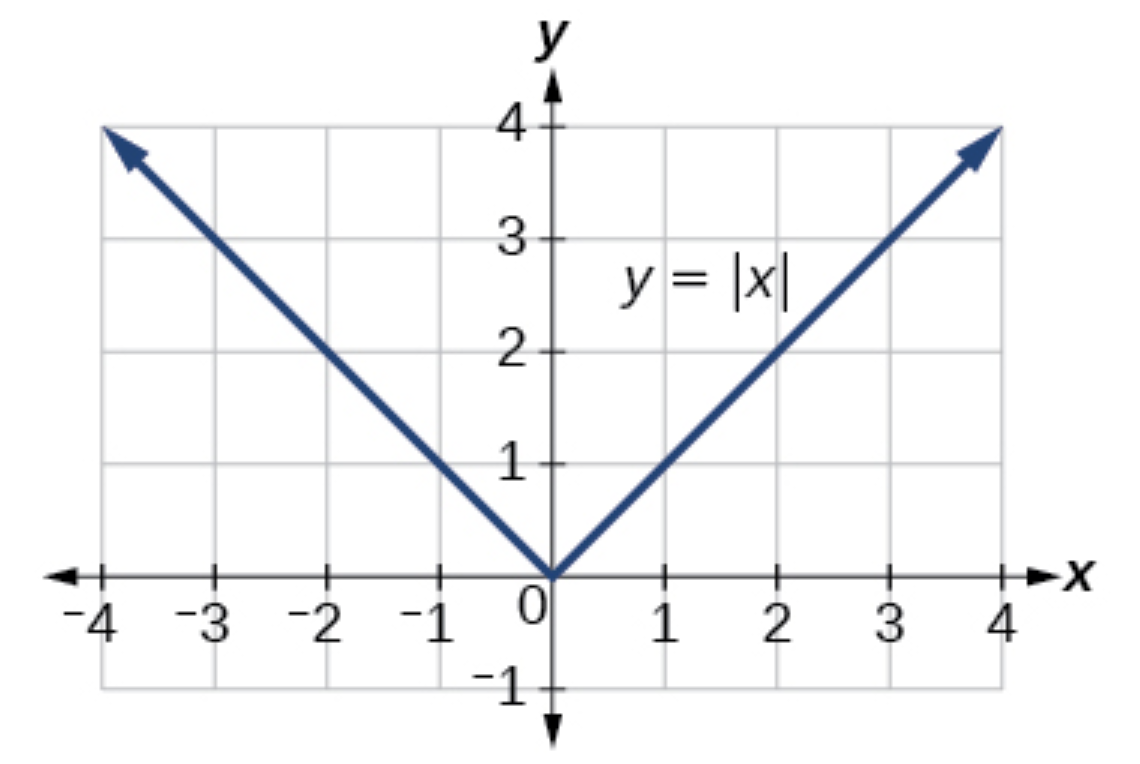
\includegraphics[width=0.5\textwidth]{images/abs_value.png}	
\end{figure}

	\begin{itemize} \footnotesize  
		\item [a.] No. For example, $f(1) = f(-1) = 1$.  Hence, distinct inputs map to the same output.
		\item [b.] Yes.  Recall that $\mathbb{N} \defeq \set{0,1,2,3, \hdots}$. We can see from the plot that all of $\mathbb{N}$ is \enquote{hit} by $f$.  For a more formal argument, we need to show that for each $n \in \mathbb{N}$, there is a $z \in \mathbb{Z}$  such that $f(z)=n$. This is easily satisfied by taking $z=n$ (or, for that matter $z=-n$).
	\end{itemize}

\end{frame}


\begin{frame}{Solution to group exercise \#3}
\footnotesize 
\textbf{Problem.} Consider the \enquote{shifting} (or translation) function $f: \mathbb{Z} \to \mathbb{Z}$ given by $f(z) = z+k$ for some fixed $k \in \mathbb{Z}$.  For instance $f(z) = z+2$ shifts all integers two units to the right.   (a) Prove that $f$ is a bijection. (b) Express the inverse function $f^{-1}$ with an explicit formula.  
%	\begin{itemize} \footnotesize 
%		\item [a.] Prove that $f$ is a bijection.
%		\item [b.] Express the inverse function $f^{-1}$ with an explicit formula.
%	\end{itemize} 
\vfill
\textbf{Solution.}
\vspace{-0.2cm}
	\begin{itemize} \footnotesize 
		\item [a.] To show that $f$ is a bijection, we need to show that it is injective and surjective.
		\begin{itemize} \footnotesize 
		\item \boxed{\text{Injective.}}  By definition, a function $f$ is injective if $a \neq a'$ implies $f(a) \neq f(a')$.  We verify this statement by contraposition. That is, we prove the logically equivalent statement that $f(a) = f(a')$ implies $a =a'$. Now 
		\[f(a) = f(a') \implies a+k = a'+k \implies a=a'. \] 
		\item \boxed{\text{Surjective.}}  By definition, a function $f$ is surjective if for any $b$ in the codomain of the function, there is an $a$ in the domain such that $f(a)=b$.  Now note that we can obtain any $b \in \mathbb{Z}$ as $b=f(a)$ by setting $a=b-k$.
		\end{itemize} 
		\item [b.] We can define $f^{-1}$ by the mapping $f^{-1}(z) = z-k.$
	\end{itemize} 
\vfill 
\begin{myredbox}[title=Remark: Proof by contraposition]
Earlier in the course, we showed that $A \implies B$ is logically equivalent to $(\texttt{not } B) \implies (\texttt{not } A)$.  (For example, this can be shown by truth tables.)  The transformed proposition is called the \underline{contrapositive}. It may be easier to prove the contrapositive form of the statement, as we did above.
\end{myredbox}

\end{frame}

\begin{frame}{Solution (Part I) to group exercise \#4}
\scriptsize 
\begin{minipage}{0.5\textwidth}
\textbf{Problem.}  Consider the \enquote{zigzag} function $f: \mathbb{N} \to \mathbb{Z}$ given by 
	\[ f(n) = 
	\begin{cases}
	\frac{n}{2}, & \text{ if $n$ is even} \\
	-\frac{n+1}{2}, & \text{ if $n$ is odd} \\
	\end{cases}
	\]
	This function \enquote{zigzags} the integers like this
	\[ 0 \to 0, 1 \to -1, 2 \to 1, 3 \to -2, \hdots \]
	Prove that $f$ is a bijection.	
\end{minipage}
\hfill 
\begin{minipage}{0.48\textwidth}
\begin{figure}
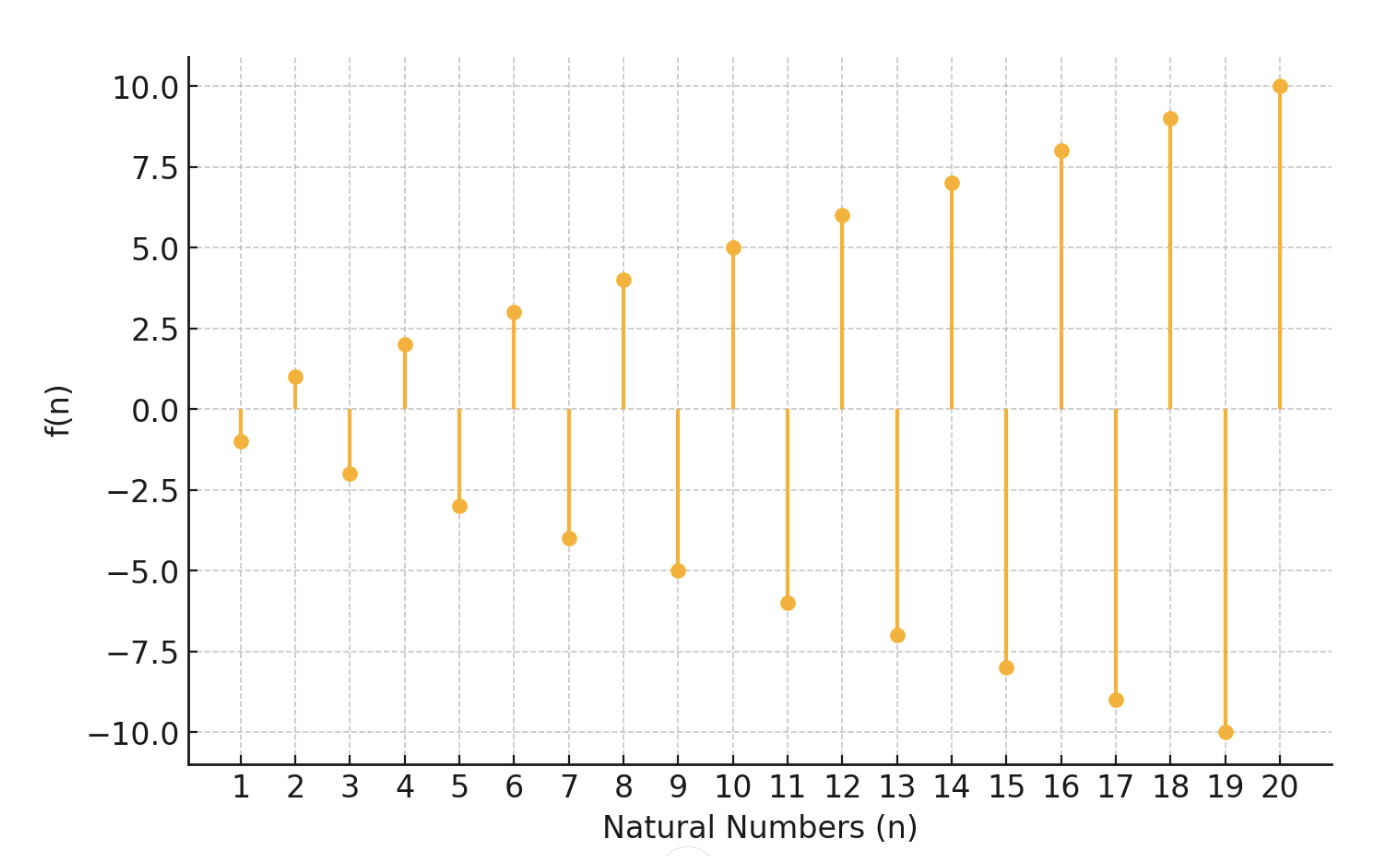
\includegraphics[width=0.95\textwidth]{images/zig_zag_function.png}	
\end{figure}
\end{minipage}
\vfill 
\textbf{Solution.}
To show that $f$ is a bijection, we need to show that it is injective and surjective.
		\begin{itemize} \scriptsize 
		\item \boxed{\text{Injective.}}  As with exercise \#3a, to prove that $f$ is injective, we show that  $f(n) = f(n')$ implies $n =n'$. First note that if $f(n)=f(n')$, then $n$ and $n'$ must have the same parity, or else $f(n)$ and $f(n')$ would have different signs.  Now
		\begin{itemize} \scriptsize 
		\item Suppose $n$ and $n'$ are both even.  Then 
		\[ f(n) = f(n') \implies \frac{n}{2} = \frac{n'}{2} \implies n=n'. \]
		\item Suppose $n$ and $n'$ are both odd.  Then 
		\[ f(n) = f(n') \implies -\frac{n+1}{2} = -\frac{n'+1}{2} \implies n=n'. \]
		\end{itemize} 
				\item \boxed{\text{Surjective.}} See next page.
		\end{itemize}
\end{frame}

\begin{frame}{Solution (Part II) to group exercise \#4}
\scriptsize 
\begin{minipage}{0.5\textwidth}
\textbf{Problem.}  Consider the \enquote{zigzag} function $f: \mathbb{N} \to \mathbb{Z}$ given by 
	\[ f(n) = 
	\begin{cases}
	\frac{n}{2}, & \text{ if $n$ is even} \\
	-\frac{n+1}{2}, & \text{ if $n$ is odd} \\
	\end{cases}
	\]
	This function \enquote{zigzags} the integers like this
	\[ 0 \to 0, 1 \to -1, 2 \to 1, 3 \to -2, \hdots \]
	Prove that $f$ is a bijection.	
\end{minipage}
\hfill 
\begin{minipage}{0.48\textwidth}
\begin{figure}
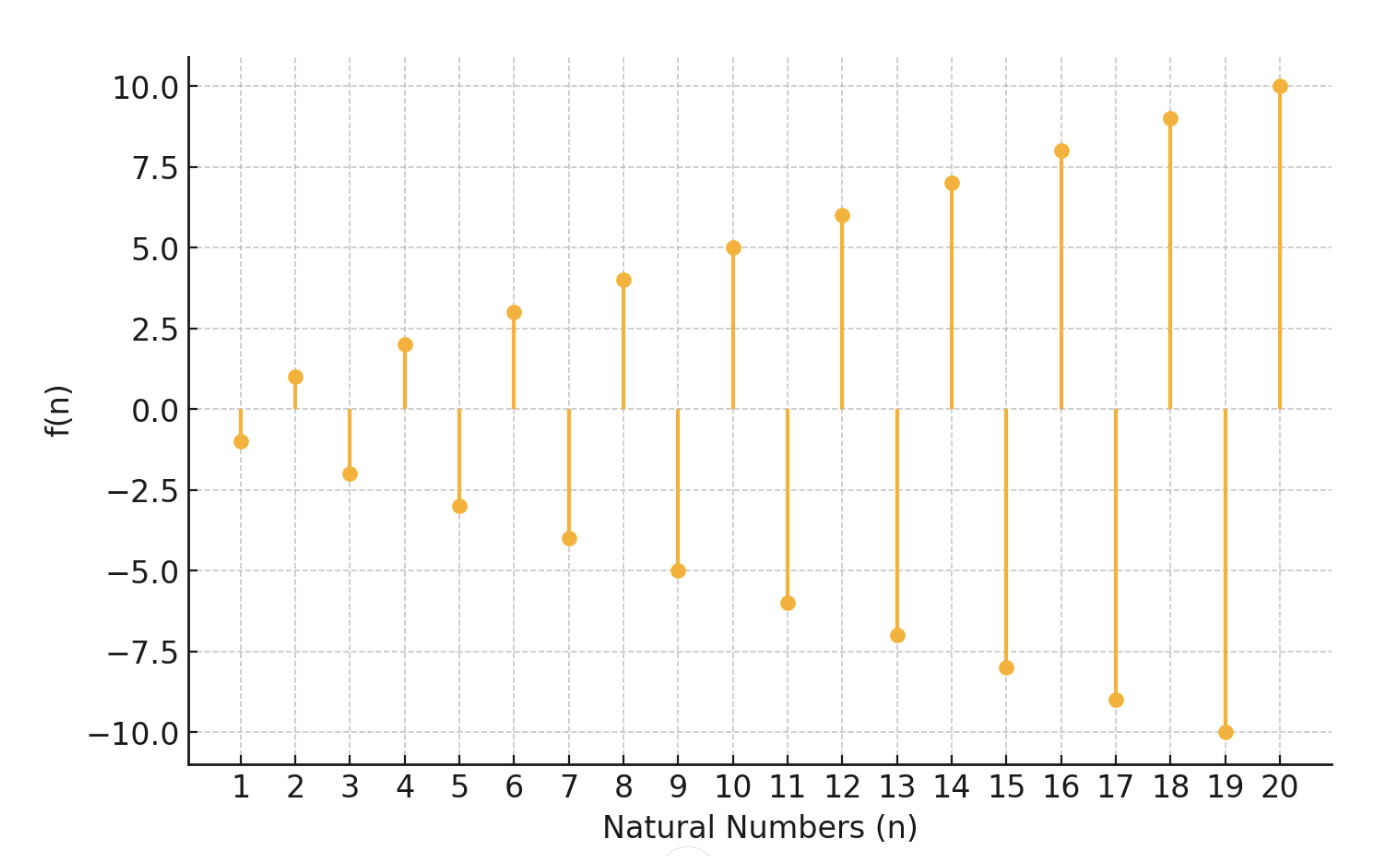
\includegraphics[width=0.95\textwidth]{images/zig_zag_function.png}	
\end{figure}
\end{minipage}
\vfill 
\textbf{Solution.}
To show that $f$ is a bijection, we need to show that it is injective and surjective.
		\begin{itemize} \scriptsize 
		\item \boxed{\text{Injective.}} See previous page.
		\item \boxed{\text{Surjective.}}  By definition, a function $f$ is surjective if for any $z \in \mathbb{Z}$, there is an $n \in \mathbb{N}$ such that $f(n)=z$.  We proceed by cases.  If $z=0$, then we take $n=0$.  If $z>0$, then we take $n=2z$.  If $z<0$, then we take $n=-2z-1$.
		\end{itemize} 
\vfill 

\begin{myredbox}[title=Remark: The strangeness of infinity]
Sets with infinitely many members have some strange properties. If $f: A \to B$ where $A$ and $B$ are finite, then $f$ being a bijection requires $|A|=|B|$.  Intuitively, each member in $A$ can't have exactly one \enquote{buddy} in $B$  unless $A$ and $B$ are the same size.  Here, however, we see that $f$ gives a bijection between $\mathbb{N}$ and $\mathbb{Z}$, even though  $\mathbb{N}$ is \enquote{smaller} than $\mathbb{Z}$ (in the sense that $\mathbb{N} \subsetneq \mathbb{Z}$).
\end{myredbox}

\end{frame}




\end{document}
